% !TeX root = ../main.tex

\chapter{实验结果}
\label{cha:experiments}

本章报告系统在两个评测集上的实验结果：自建中文评测集（80条）和TextVQA 0.5.1公开验证集（采样50条），并对结果进行对比分析。所有实验均使用DashScope平台的Qwen3-VL-Flash模型完成。

\section{实验设置}

\subsection{自建评测集}

自建评测集包含80条中文问答数据，覆盖两大类五个子类别：

\begin{table}[htbp]
  \centering
  \caption{自建评测集构成}
  \label{tab:self_dataset}
  \begin{tabular}{|l|l|r|}
    \hline
    \textbf{类别} & \textbf{子类别} & \textbf{数量} \\
    \hline
    \multirow{5}{*}{自然场景（40条）} & recognition（物体识别） & 26 \\
    \cline{2-3}
     & attribute（属性描述） & 8 \\
    \cline{2-3}
     & reasoning（推理判断） & 6 \\
    \hline
    \multirow{2}{*}{文档图像（40条）} & ocr（文字识别） & 27 \\
    \cline{2-3}
     & summary（文档摘要） & 13 \\
    \hline
    \textbf{合计} & & \textbf{80} \\
    \hline
  \end{tabular}
\end{table}

\subsection{公开评测集}

从TextVQA 0.5.1验证集（5000条）中按固定随机种子（seed=42）抽取50条，通过flickr\_300k\_url字段下载对应图片。TextVQA的每条数据包含10个标注者答案，采用"任一答案命中即判正确"的标准评测方式。

\subsection{评测方法}

自建集采用基于jieba中文分词的语义匹配算法：提取期望答案的内容词，统计模型回答中的命中情况。短答案（$\leq$3个内容词）需命中全部或至少2个词且不含否定词；长答案匹配率需$\geq$40\%。公开集采用英文大小写不敏感的字符串包含匹配。

\section{自建集评测结果}

\subsection{总体结果}

\begin{table}[htbp]
  \centering
  \caption{自建集总体评测结果}
  \label{tab:self_overall}
  \begin{tabular}{|l|r|}
    \hline
    \textbf{指标} & \textbf{值} \\
    \hline
    总数据量 & 80 \\
    匹配数 & 44 \\
    错误数 & 0 \\
    \textbf{整体准确率} & \textbf{55.0\%} \\
    平均响应时间 & 2.80s \\
    \hline
  \end{tabular}
\end{table}

\subsection{分类结果}

\begin{table}[htbp]
  \centering
  \caption{按类别统计}
  \label{tab:self_category}
  \begin{tabular}{|l|r|r|r|}
    \hline
    \textbf{类别} & \textbf{数据量} & \textbf{准确率} & \textbf{平均响应时间} \\
    \hline
    自然场景 & 40 & 52.5\% & 3.69s \\
    文档图像 & 40 & 57.5\% & 1.90s \\
    \hline
  \end{tabular}
\end{table}

\begin{table}[htbp]
  \centering
  \caption{按子类别统计}
  \label{tab:self_subcategory}
  \begin{tabular}{|l|r|r|}
    \hline
    \textbf{子类别} & \textbf{数据量} & \textbf{准确率} \\
    \hline
    attribute（属性描述） & 8 & 75.0\% \\
    ocr（文字识别） & 27 & 63.0\% \\
    reasoning（推理判断） & 10 & 60.0\% \\
    recognition（物体识别） & 26 & 46.2\% \\
    summary（文档摘要） & 9 & 33.3\% \\
    \hline
  \end{tabular}
\end{table}

\subsection{结果分析}

自建集55.0\%的准确率是在修复评测算法虚高问题（旧算法因短答案"命中1词即判OK"的宽松策略导致81.2\%的虚高准确率）后得到的更真实的结果。关键发现：

\begin{itemize}
  \item \textbf{文档图像（57.5\%）略优于自然场景（52.5\%）}：文档OCR类问题答案较为固定（日期、标题等），模型判断相对准确；自然场景需要更复杂的语义理解；
  \item \textbf{属性描述表现最好（75.0\%）}：颜色、数量等客观属性问题难度较低，模型理解准确；
  \item \textbf{摘要总结表现最差（33.3\%）}：需要模型从文档中提取核心信息并归纳，涉及更高层次的语言理解能力；
  \item \textbf{物体识别存在系统性问题}：大量失败案例源于模型正确回答"图中没有XX"但与期望的肯定答案矛盾，反映出评测集中部分问题假设过强的问题。
\end{itemize}

\section{公开集评测结果}

\subsection{总体结果}

\begin{table}[htbp]
  \centering
  \caption{TextVQA公开集评测结果}
  \label{tab:public_overall}
  \begin{tabular}{|l|r|}
    \hline
    \textbf{指标} & \textbf{值} \\
    \hline
    采样数 & 50 \\
    有效样本 & 36 \\
    跳过（图片下载失败） & 14 \\
    匹配数 & 31 \\
    \textbf{准确率} & \textbf{86.1\%} \\
    平均响应时间 & 1.70s \\
    \hline
  \end{tabular}
\end{table}

有效样本36条（$\geq$30），结果具有统计意义。14条图片因Flickr外链自然过期（HTTP 404/410）被跳过。

\section{对比分析}

\subsection{自建集与公开集对比}

\begin{table}[htbp]
  \centering
  \caption{自建集与TextVQA公开集对比}
  \label{tab:comparison}
  \begin{tabular}{|l|r|r|}
    \hline
    \textbf{维度} & \textbf{自建集} & \textbf{TextVQA公开集} \\
    \hline
    准确率 & 55.0\% & 86.1\% \\
    平均响应时间 & 2.80s & 1.70s \\
    语言 & 中文 & 英文 \\
    主要题型 & 场景理解/推理/OCR/摘要 & OCR文字阅读为主 \\
    样本量 & 80（全有效） & 36有效/50采样 \\
    评测匹配算法 & jieba分词+否定词检测 & 字符串包含匹配 \\
    \hline
  \end{tabular}
\end{table}

两个评测集的准确率差异（31.1个百分点）主要由以下因素导致：

\begin{enumerate}
  \item \textbf{任务类型差异}：TextVQA以"图片中写了什么文字"类OCR题为主，Qwen3-VL-Flash对此类任务擅长；自建集涵盖自然场景理解、推理判断、文档摘要等更广泛的语义理解题型，难度更高；
  \item \textbf{语言差异}：TextVQA为英文题，模型在大规模英文数据上预训练充分；自建集为中文题，中文VLM的理解和生成能力仍有提升空间；
  \item \textbf{匹配算法差异}：TextVQA使用简单的字符串包含匹配（10个标注者答案任一命中即OK），宽松度较高；自建集使用jieba分词+否定词检测+阈值判定，匹配条件更严格。
\end{enumerate}

\subsection{可视化分析}

图\ref{fig:category_accuracy}展示了自建集两个类别与公开集的准确率对比，直观呈现了任务类型差异对模型表现的显著影响。

\begin{figure}[htbp]
  \centering
  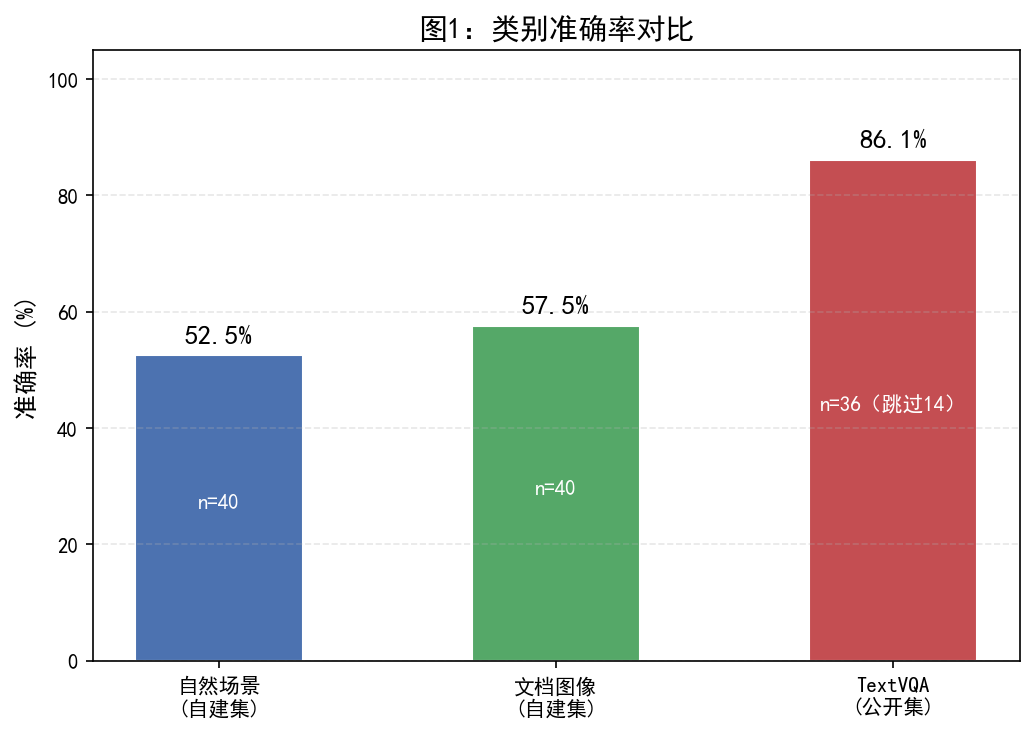
\includegraphics[width=0.85\textwidth]{../../evaluation/figures/category_accuracy.png}
  \caption{类别准确率对比}
  \label{fig:category_accuracy}
\end{figure}

图\ref{fig:subcategory_accuracy}进一步分解了自建集五个子类别的表现差异。摘要总结（summary, 33.3\%）和物体识别（recognition, 46.2\%）是当前模型的最薄弱环节。

\begin{figure}[htbp]
  \centering
  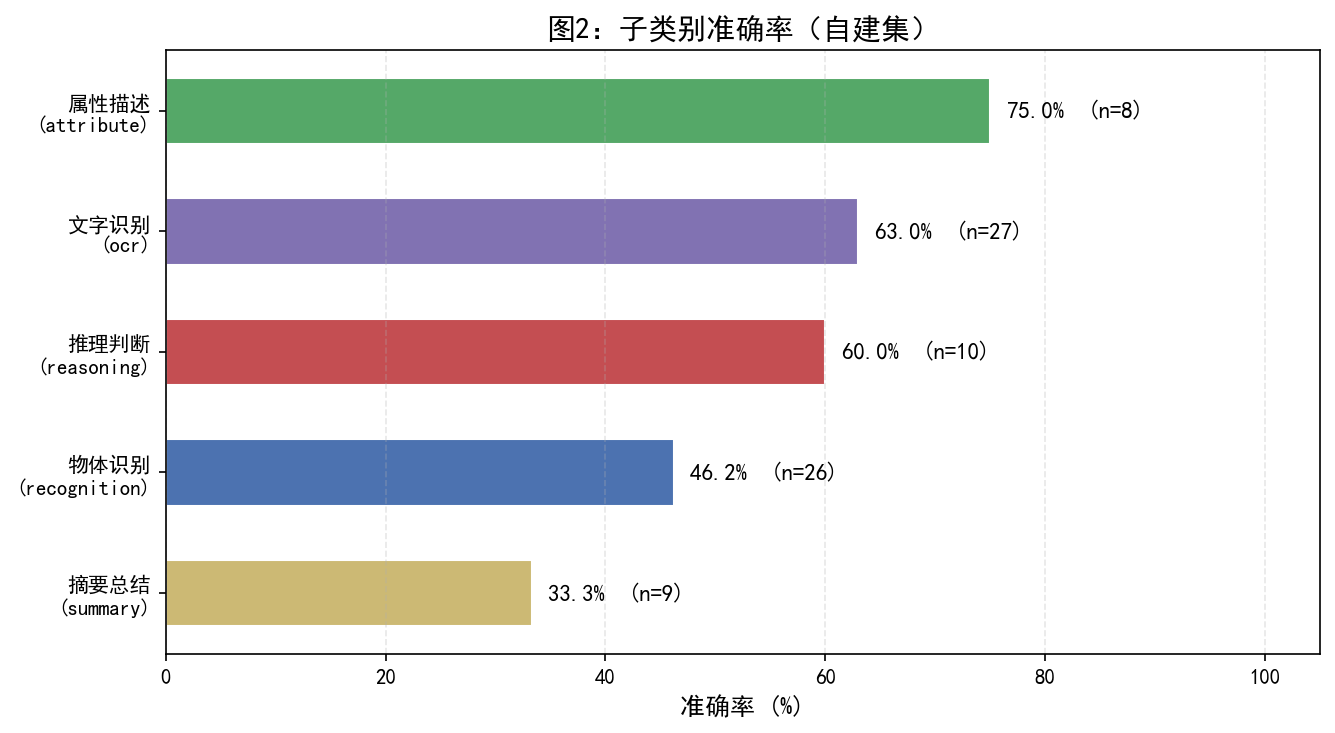
\includegraphics[width=0.85\textwidth]{../../evaluation/figures/subcategory_accuracy.png}
  \caption{子类别准确率（自建集）}
  \label{fig:subcategory_accuracy}
\end{figure}

图\ref{fig:response_time}展示了自然场景与文档图像两类问题的响应时间分布。文档图像的响应时间中位数（约1.5s）明显低于自然场景（约3.0s），且自然场景存在多个长尾慢响应（6s以上），反映出不同难度问题对模型推理时间的显著影响。

\begin{figure}[htbp]
  \centering
  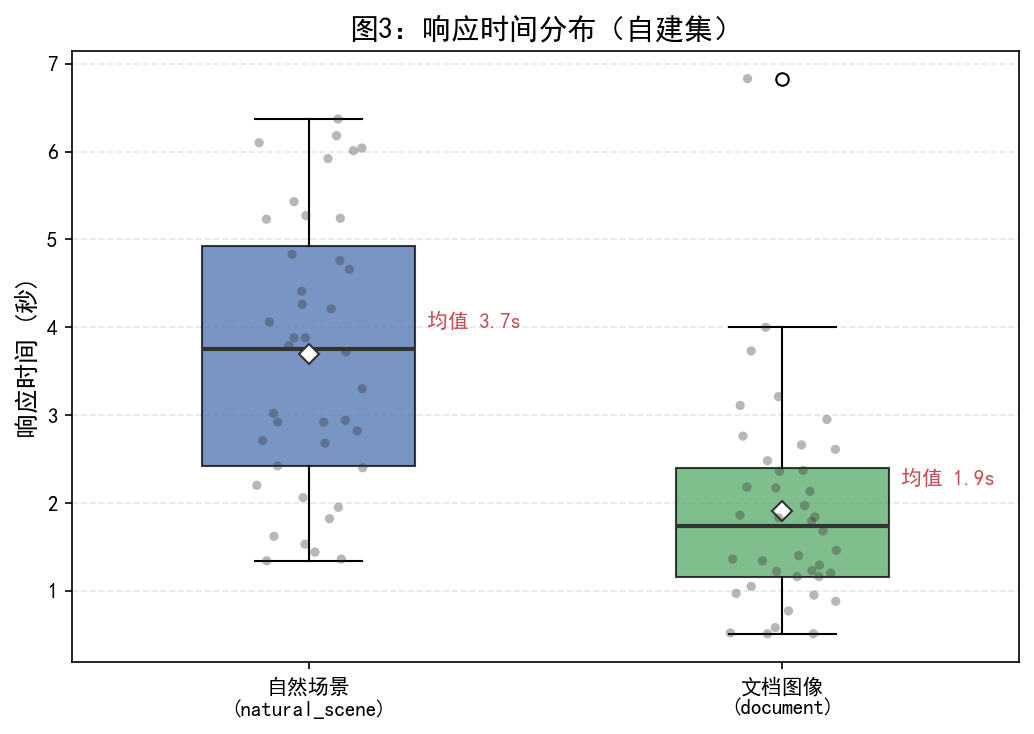
\includegraphics[width=0.85\textwidth]{../../evaluation/figures/response_time.png}
  \caption{响应时间分布（自建集）}
  \label{fig:response_time}
\end{figure}

\section{小结}

本章通过自建集（80条中文）和TextVQA公开集（36条有效英文）的双轨评测，获得了对Qwen3-VL-Flash模型能力的较全面认识。自建集55.0\%的准确率更真实地反映了模型在中文多模态语义理解上的当前水平，而TextVQA 86.1\%的高准确率验证了其在英文OCR类任务上的突出能力。下一章将选取典型成功与失败案例进行深度分析。
